%!TEX root = ../document.tex
\chapter{Empirical settings and methods}
In this chapter...

\section{Empirical setting}
The collection of data material used in this thesis took part in the late autumn, 2013, at a high school located in the centre of Oslo. The school is in the upper third on the grade scale, with a limit of 43.5 points for admission in 2010/2011 \citep{utdanningsetaten}. Therefore the students at this school are mostly high achievers. 

Contact with the school was first initiated through Intermedia, and a presentational flyer was sent as an explanation of the project (_____appendix_____). Luckily our request coincided perfectly with a 2 week time frame for reviewing photosynthesis in one of the teacher's classes, and he was therefore quite eager to use our application in class. 

The class selected for the experiment was a biology class at the highest level offered at the school, biologi 2, which has an extensive curriculum covering e.g photosynthesis, enzymes and energy transmitters. The students were between 17 and 18 years of age, and for the main part most of the 20 students taking the class were present. All the students aggred to participate in the study, but due to technical limitations, data collection was only done with a small sample of the group. 


\def\arraystretch{1.8}
\begin{table}
    \begin{tabular}{@{}lp{250pt}@{}}\toprule
    Sensor               & Description \\ \midrule                                                                                                  
    TSL2561              & Digital luminosity sensor. Measures light in lux from 300-1100nm.                                            \\ 
    RHT03                & Digital humidity and temperature sensor. Measures relative humidity and temperature in celsius.              \\ 
    DS18B20              & Digital waterproof temperature sensor. Measures temperature in celsius                                       \\ 
    DFRobot sku:sen0114  & Analog soil moisture sensor. Returns values between 0 and 900 depending on electrical conductivity of soil.  \\ \bottomrule
    \end{tabular}
    \caption{Sensors used in the application}
\end{table}


With the advent of the \emph{“internet of things”}, sensors are becoming available in many different forms and packages. Just as LEGO-pieces they can be used in a wide range of applications. From automating tasks such as keeping a steady indoor-temperature, to measuring variables which we as humans cannot see. 

For this application we did a short review of the available off-the-shelf packages available on the market. 

The sensors are able to capture information about the environment and transform it to data variables which we can store and categorize. In total there are five different sensors connected to the plant, or in the plant’s vicinity: soil moisture, soil temperature, air temperature, humidity, and light. 


(write something about the sensortag)

Simplified we can say that the sensors function in the same way as a volume controller on an amplifier. On an amplifier one can adjust the volume by varying the resistance in the signal going to the speakers. If we turn the volume up, the resistance goes down, which lets more power through to the speakers. And if we turn the volume down, the resistance goes up which lets less power flow to the speakers. The concept with sensors is the same, only that instead controlling resistance with a volume knob, it is controlled by light, moisture or other environmental variables. 

For a good example, lets look at how the temperature sensors work. The resistors used in the temperature sensors are called “thermistors”, and the way they operate is by varying the resistance according to the temperature. Since we already know how many volts we are sending to the thermistor on the one end, we can use the amount of volts we get back to calculate the resistance. In our application this is done by a voltage divider which uses a formula as follows: 

\begin{equation}
U_{out}=\frac{R_{2}}{R_{1}+R_{2}}\cdot U_{in} 
\label{eq:vdiv1}
\end{equation}
Where $V_{out}$ is voltage out, $U_{in}$ is voltage in, $R_{1}$ is a given resistance, and $R_{2}$ is the resistance we want to calculate. For this example let's assume that $U_{in} = 5_{v}$, $U_{out} = 2_{v}$, and $R_{1} = 1K\Omega$. We solve this equation with regard to $R_{2}$
\begin{equation}
R_{2} = \frac{U_{out} \cdot R_{1}}{U_{in}-U_{out}}
\end{equation} 

\begin{equation}
R_{2} = \frac{2V \cdot 1000\Omega}{5V-2V}
\end{equation} 

\begin{equation}
R_{2} = \frac{2000\Omega}{3}
\end{equation} 

\begin{equation}
R_{2} = 667\Omega
\end{equation} 

Then we can see that the calculated resistance is 667$\Omega$. This value can then be mapped to the correct unit of measure, in this case Celsius or Fahrenheit. 

As we are using digital sensors, all of these calculations are done internally in the sensors, and coded into a digital signal. This signal, consisting of 1s and 0s, is then passed onto the next unit in our system, the Arduino.  

\subsection{Arduino}
(Write about embedded systems. What other alternatives are there to the Arduino? )

Arduino is an open-source prototyping platform which makes it easy to interface low-level electronics (e.g sensors) with higher-level electronics (e.g computers). The core part of the Arduino is an Atmel\texttrademark Atmega microcontroller which can be programmed by a computer over usb, using the Arduino programming language and the Arduino development environment \citep{arduino}.

We have used an Arduino Uno which has 13 digital input output pins (GPIO), five analog inputs, i2c inputs, and USB for serial communication. The DSB18B20 soil temperature sensor and RHT03 temperature and humidity sensor are connected to the digital inputs through a 1K(ohm) pullup resistor. The pullup resistors are used to keep the voltage sent to the arduino from fluctuating when the sensor is not sending any data. The TSL2561 luminosity sensor is connected to the A4/SDA and A5/SDL ports of the Arduino as it communicates over the i2c protocol. And the DFRobot soil moisture sensor is connected to A3 (Analog input 3) as it outputs analog voltage.  

\begin{figure}
\centering
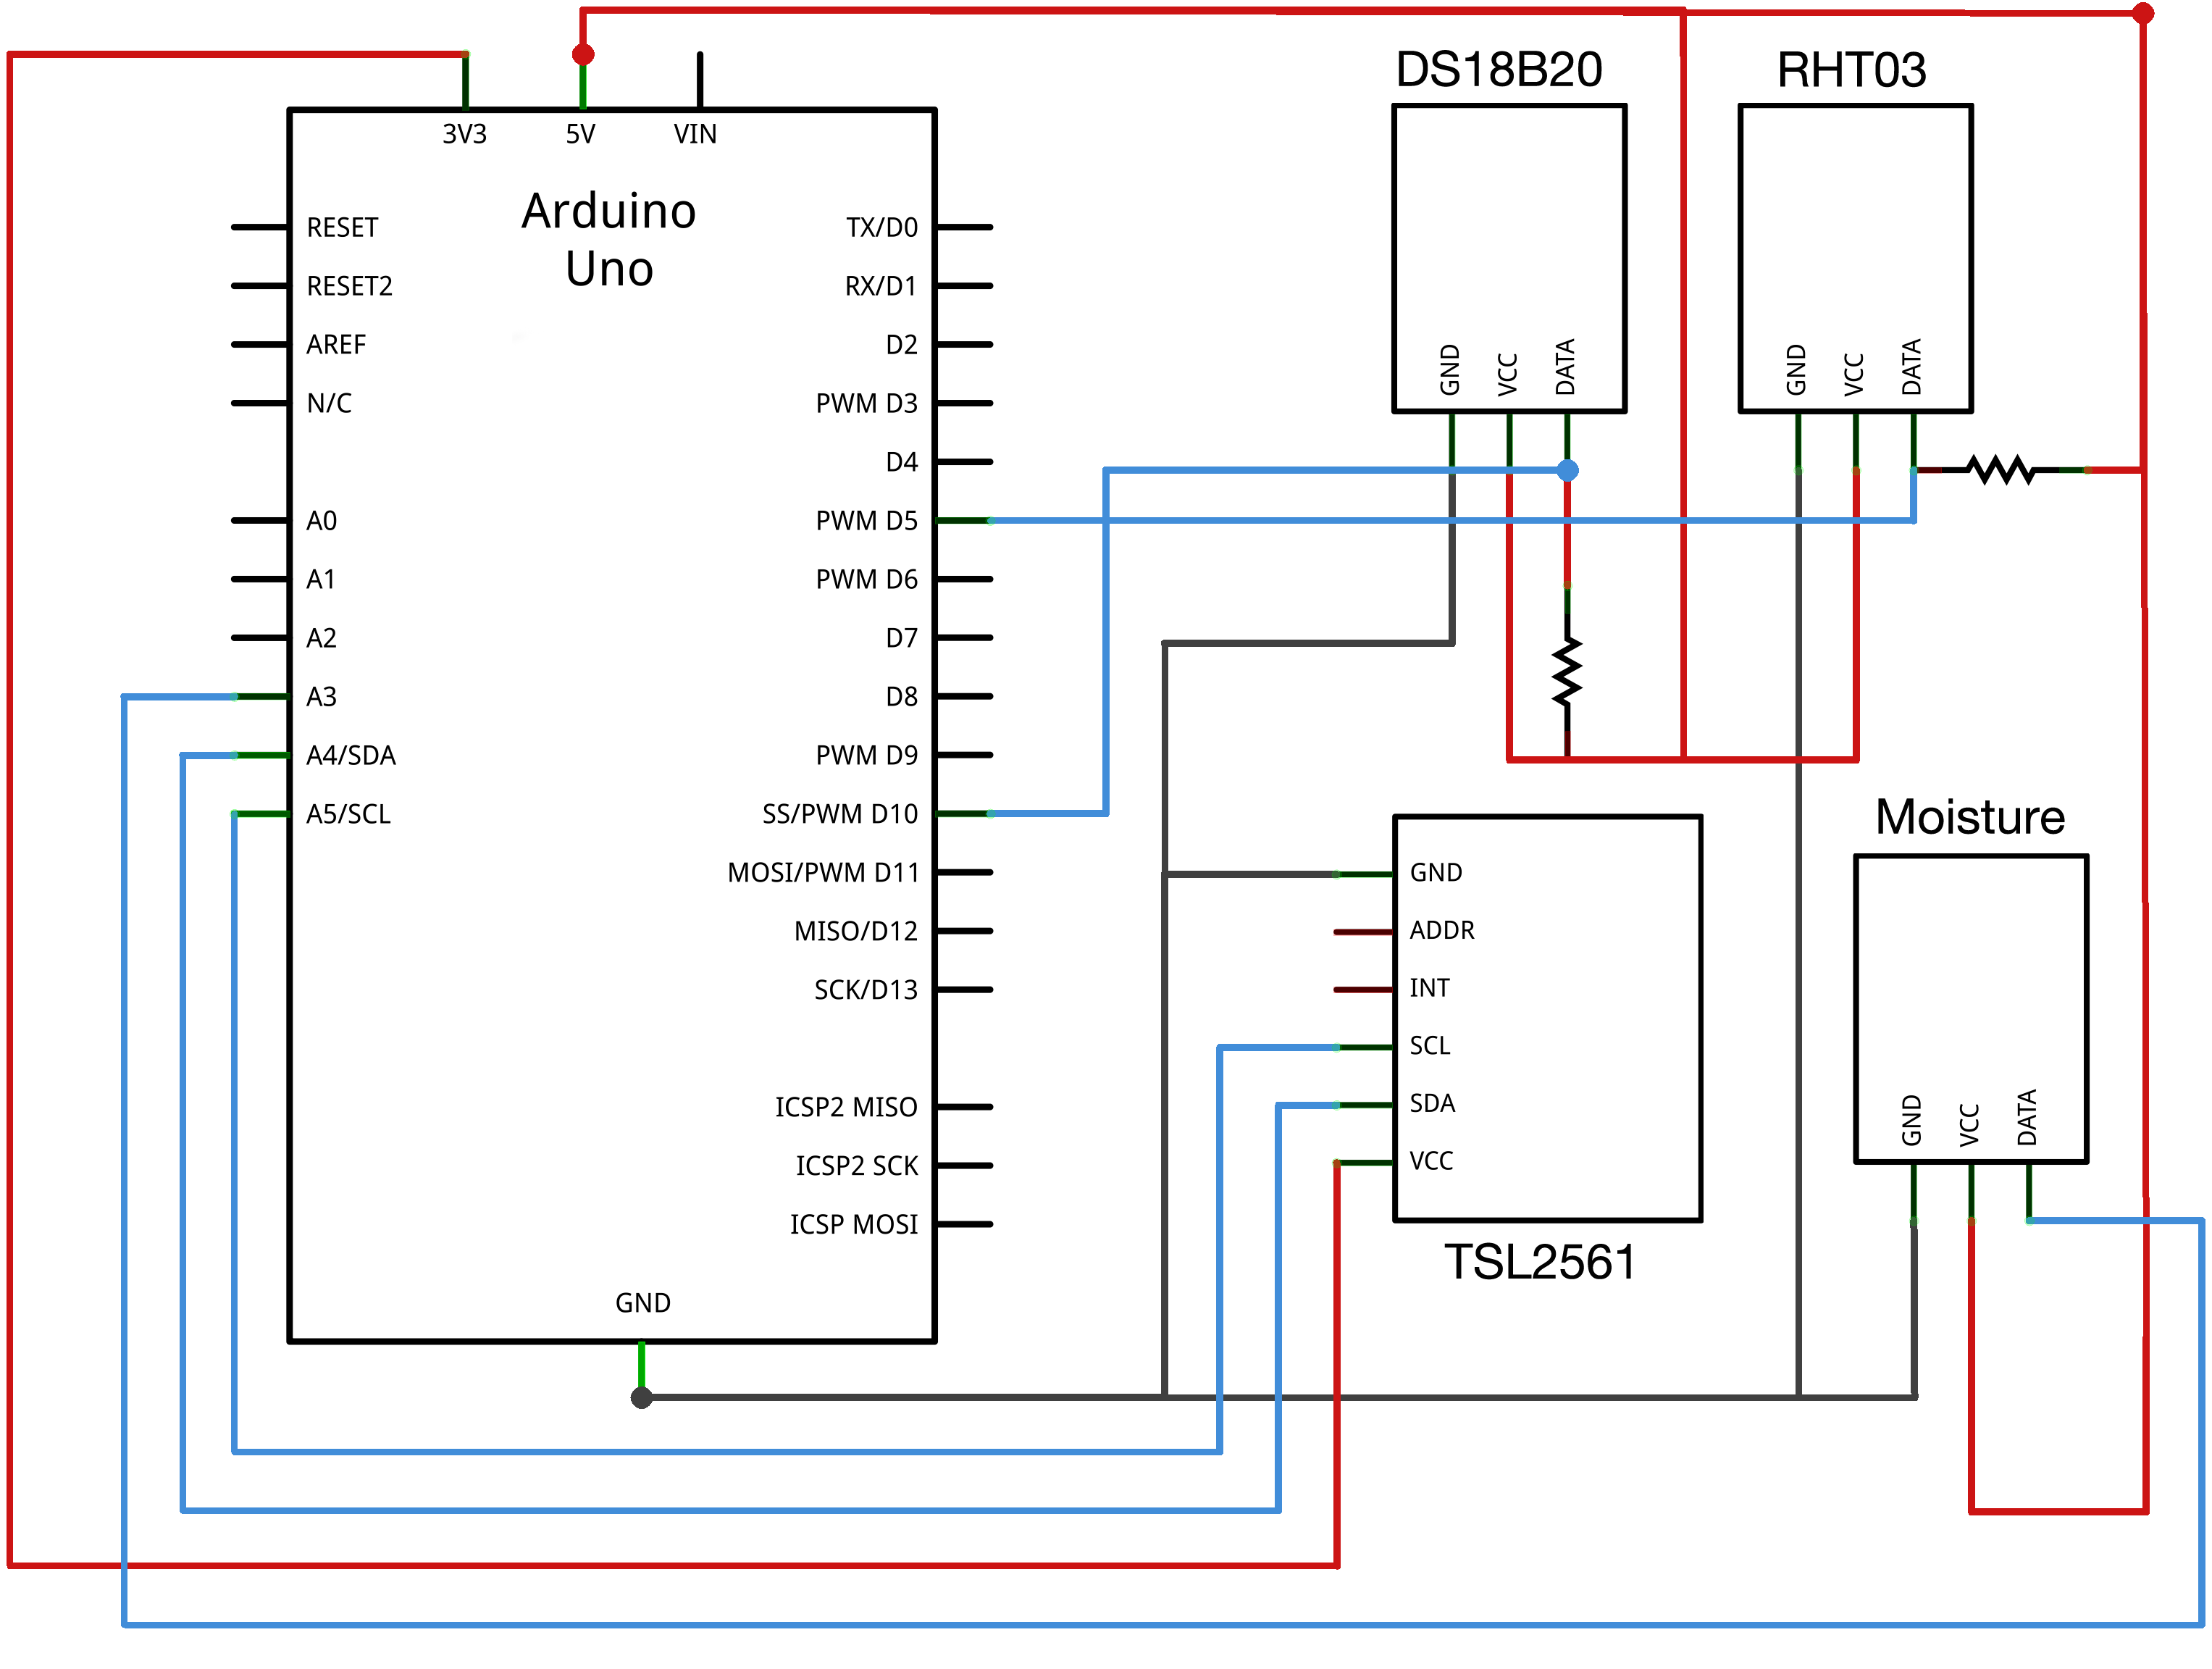
\includegraphics[width=1\textwidth]{img/hardware/Arduino_and_sensors_schem.png}
\caption{Schema diagram of Arduino sensor wiring}
\label{fig:arduino}
\end{figure}

The community surrounding Arduino is quite large, and therefore we were able to find pre-written libraries for communicating with the different sensors. This has made the task of converting the digital signal to the correct units (celsius, relative humidity, lux) and levels a breeze. 

In the case of the soil moisture sensor, it does not output soil moisture in any kind of universal unit. Therefore we measured the resistance in air (high resistance), and in water (low resistance), and let these be the high and low points of a new unit called arbitrary moisture units (AMU).

The code residing in the arduino runs a simple loop where it waits for a special character sent over serial communication through USB. If it receives this character it reads all the sensor values, and sends them back to the next logical unit: the Raspberry Pi

\subsection{Raspberry Pi}
(Why raspberry? Beagleboard?)
The Raspberry Pi is a “cheap, accessible, programmable computer” \citep{raspberrypi} which is roughly the size of a credit card. Our model was released early 2012, and contains two usb ports, audio, sd-card slot, and several GPIO-pins. The devices connected to it are: wireless network adapter, high-definition webcamera, and the Arduino. The operating system running on it is a port of Debian Linux optimized for the Raspberry, called Raspbian. 

(illustration of raspberry)

The GPIO-pins on the raspberry works almost in the same fashion as the Arduino’s digital input output pins. Thus we could in theory simplified the hardware by omitting the Arduino. The main reason for not doing this is that the Raspberry does not have an analog to digital converter (ADC). Therefore we would have to make a complex circuit involving an ADC to interface the Raspberry with the soil moisture sensor. In addition, we would most likely face timing issues. When we ask the digital sensors for data, they send the response immediately. If the unit receiving is not available to read the data, it gets lost. This can be a problem when using a high-level computer, as it performs multiple other tasks in addition to reading sensordata. 

\subsubsection{Operation}
After booting up an endless loop bash-script is called. The script snaps a photo of the plant using the webcam, and then runs a python-script responsible for collecting sensordata. Since we sometimes can get erroneous values from the sensors, we read 15 values and upload the median value.

%http://en.wikibooks.org/wiki/LaTeX/Packages/Listings
\lstset{language=Python} 
\begin{figure}
\begin{lstlisting}
//instantiate lists
airtemp = []
humidity = []
light = []
soiltemp = [] 

for x in xrange(1,15): 
	ser.write("r") //Ask Arduino for data
	variables = ser.readline() //Read the data
	sensorReadings = variables.split('|') //Split string on |

	airtemp.append(float(sensorReadings[0]))
	humidity.append(float(sensorReadings[1]))
	light.append(float(sensorReadings[2]))
	soiltemp.append(float((sensorReadings[3])[:-2])) 

//calculate and post the median using numpy
postData(np.median(airtemp),np.median(humidity),np.median(light),np.median(soiltemp)) 
\end{lstlisting}
\caption{Reading sensor values from Arduino on Raspberry PI}
\label{fig:raspberrycode}
\end{figure}

These values, along with the photo of the plant, are then passed on to the next instance, the API, using pythons HTTP-library urllib2. 

\section{Data processing and database}
When the data has been gathered at the low level hierarchy, it is stored in the cloud. This is done by posting the data to an API on our web server. The main function of an API is to be a mean of communication between software, in our case the data collector and the user interface. After some research on web-API design, we decided that a REST architectual style was the way to go. 

\subsection{Representational State Transfer (REST)}
REST is an architectual style for distributed hypermedia systems \citep{fielding2000architectural}. In Fielding's dissertation, he writes about the interaction constraints of REST that is introduced in order to limit how a distributed system can be constructed. 
=======
\subsection{Planning}
The planning of the project was done by us in conjuction with the teacher responsible for the for the biology class. An initial plannign meeting was held at the school around one week before the experiments started. There we gave the teacher a thorough introduction of the system, and presented some ideas for expirements the students could perform using our system as platform. This involved:
>>>>>>> 4056fd08d59c7d41cdee9e1f90c94e5ae23dbd4d

\begin{enumerate}
\item{Present the application in class}
\item{Initiate an experiment using the application. Related to e.g soil moisture, light intensity, light quality, or temperature}
\item{Have a one hour session where the students work with text tasks realted to the experiment}
\end{enumerate}

The teacher then suggested that we could conduct two experiments, so the students could work on the relations between the different external factors effect on photosynthesis. As the system records a range of different variables, it would be possible to keep the environment relatively controlled, or at least point to factors which could be sources of error in the experiment. 

We agreed that the factor where we could get the most interesting result was to vary the light intesity and the light quality (wavelength). The first experiment would then involve keeping the plant located in a window facing west, receiving sunlight and light from the fluorescent indoor-lighting. In the second experiment we would plant new seeds, and relocate the plant to a (presumably) light proof cupboard. The plant would then only be given green light, with a known wavelength. Each of the experiments would have a duration of approximately one week. 

\subsection{Execution pow pow ?}
The project was presented and the first experiment initiated by one of the students on friday 25th of october. This went on until friday 1st of november when the second experiment was initiated. The second experiment went on until wednesday 13th of november when the primary data collection session started. During the experiments we were present at four separate occations, observing what the teacher was focusing on, and what kind of questions/which part of the photosynthesis the students found most difficult. In addition to answering questions about the system, and if/how the system was used in the education. 

\subsection{Data collection}


Our main data material consists of x hours of video from the session... blabla

\section{Analytical Procedures}

\subsection{Ethics}



